%!TEX root = ../note.tex
% Source: ../chapter2_econ101_fall2026.pdf
\section{Demand and consumer choice}
\subsection{Individual demand}
\begin{defi}
  The \term{individual demand curve} of a buyer $i$ is the function
  \[
    q_i^D : \R_{\geq 0} \to \R_{\geq 0},\qquad p \mapsto q_i^D(p),
  \]
  giving the quantity demanded at each price $p$, \emph{holding everything
  else constant} (\term{ceteris paribus}). By convention price goes on the
  vertical axis and quantity on the horizontal axis.
\end{defi}

\begin{eg}[Darren's demand for gasoline]\label{eg:darren}
  A survey of Darren's daily gas use (litres) at hypothetical prices:
  \begin{center}
    \begin{tabular}{cccccc}
      \toprule
      $p$ (\$/litre) & 2.40 & 2.20 & 2.00 & 1.80 & 1.60 \\
      $q^D_{\text{Darren}}(p)$ & 1 & 2 & 3 & 5 & 7 \\
      \bottomrule
    \end{tabular}
  \end{center}
\end{eg}

\begin{law}[Law of demand]
  Quantity demanded rises when the price falls, and vice versa:
  \[
    p_1 < p_2 \implies q^D(p_1) \geq q^D(p_2).
  \]
  That is, demand curves are \emph{downward sloping}.
\end{law}

\subsection{The rational rule for buyers}
To explain the law of demand, apply the marginal principle to a buyer who
takes the price $p$ as given. Buying the $k$-th unit has marginal benefit
$\MB(k)$ and marginal cost $p$.

\begin{nthm}[Rational rule for buyers]\label{thm:buyer}
  Suppose $\MB(1) \geq \MB(2) \geq \cdots$ (\term{diminishing marginal
  benefit}). At price $p$ the surplus-maximising quantity is
  \[
    q^D(p) = \max\set{k \geq 0 : k = 0 \text{ or } \MB(k) \geq p}
    = \#\set{k \geq 1 : \MB(k) \geq p}.
  \]
  At an interior optimum, $\text{price} = \text{marginal benefit}$.
\end{nthm}
\begin{proof}
  Apply Theorem~\ref{thm:rational} with $\MC(k) = p$ for all $k$. Since $\MB$
  is nonincreasing, the set $\set{k : \MB(k) \geq p}$ is an initial segment
  $\set{1, \ldots, q^D(p)}$, so its largest element equals its size.
\end{proof}

\begin{ncor}\label{cor:lawdemand}
  Diminishing marginal benefit implies the law of demand. Moreover, the
  demand curve \emph{is} the marginal benefit curve.
\end{ncor}
\begin{proof}
  If $p_1 < p_2$ then $\set{k : \MB(k) \geq p_2} \subseteq \set{k : \MB(k)
  \geq p_1}$, so $q^D(p_2) \leq q^D(p_1)$ by Theorem~\ref{thm:buyer}.
\end{proof}

\begin{eg}\label{eg:darren-mb}
  Darren ranks the uses of each extra litre:
  \begin{center}
    \begin{tabular}{clc}
      \toprule
      $k$ & Use of the $k$-th litre & $\MB(k)$ \\
      \midrule
      1 & drive to work instead of the bus & 2.40 \\
      2 & drive to school instead of biking & 2.20 \\
      3 & shop at the cheaper No Frills & 2.00 \\
      4 & drive to see friends & 1.90 \\
      5 & drive to the gym & 1.80 \\
      6 & drive to do errands & 1.70 \\
      7 & scenic drive & 1.60 \\
      \bottomrule
    \end{tabular}
  \end{center}
  At $p = 1.85$, $\set{k : \MB(k) \geq 1.85} = \set{1, 2, 3, 4}$, so Darren
  buys $4$ litres a day. The formula also reproduces the survey in
  Example~\ref{eg:darren}: e.g.\ at $p = 1.80$ he buys $5$ litres.
\end{eg}

\begin{center}
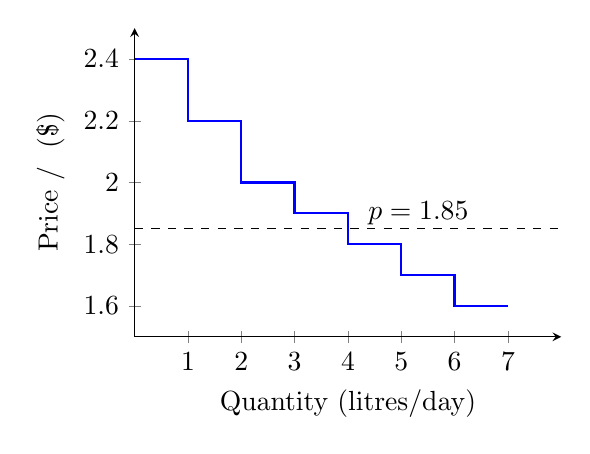
\begin{tikzpicture}
  \begin{axis}[width=7cm, height=5.5cm, xmin=0, xmax=8, ymin=1.5, ymax=2.5,
      xlabel={Quantity (litres/day)}, ylabel={Price / $\MB$ (\$)},
      axis lines=left, xtick={1,...,7}, ytick={1.6,1.8,2.0,2.2,2.4},
      yticklabel style={/pgf/number format/fixed, /pgf/number format/precision=2}]
    \addplot[const plot, thick, blue] coordinates
      {(0,2.4) (1,2.2) (2,2.0) (3,1.9) (4,1.8) (5,1.7) (6,1.6) (7,1.6)};
    \addplot[dashed] coordinates {(0,1.85) (8,1.85)};
    \node[anchor=west] at (axis cs:4.2,1.9) {$p = 1.85$};
  \end{axis}
\end{tikzpicture}
\end{center}

\subsection{Market demand}
\begin{defi}
  If the buyers are $i = 1, \ldots, N$, the \term{market demand curve} is the
  horizontal sum of the individual demand curves:
  \[
    Q^D(p) = \sum_{i=1}^{N} q_i^D(p).
  \]
\end{defi}

\begin{nprop}
  If every $q_i^D$ is nonincreasing, then so is $Q^D$.
\end{nprop}
\begin{proof}
  A sum of nonincreasing functions is nonincreasing.
\end{proof}

A movement along $Q^D$ reflects two things: existing buyers changing the
quantity they buy, and buyers entering or leaving the market ($q_i^D(p)$
changing between $0$ and a positive value).

\begin{eg}[Estimating market demand]
  Survey a random sample of $n = 400$ people from a population of
  $N = 40$ million. If $\bar q(p)$ is the average demand in the sample, then
  $Q^D(p) \approx N \bar q(p) = \frac{N}{n} \sum_{i \in \text{sample}}
  q_i^D(p)$, with scale factor $\frac{N}{n} = 100{,}000$.
  \begin{center}
    \begin{tabular}{cccc}
      \toprule
      $p$ & Sample total (litres) & $\times\, N/n$ & $Q^D(p)$ (millions) \\
      \midrule
      1.60 & 1{,}200 & $10^5$ & 120 \\
      1.80 & 1{,}100 & $10^5$ & 110 \\
      2.00 & 1{,}000 & $10^5$ & 100 \\
      2.20 & 900     & $10^5$ & 90 \\
      2.40 & 800     & $10^5$ & 80 \\
      \bottomrule
    \end{tabular}
  \end{center}
\end{eg}

\subsection{Movements along versus shifts of demand}
Demand really depends on many variables:
\[
  Q^D = Q^D(p;\ I,\ \theta,\ p_r,\ e,\ \ldots,\ N),
\]
where $I$ is income, $\theta$ preferences, $p_r$ prices of related goods,
$e$ expectations and $N$ the number of buyers. The demand \emph{curve} is
the graph of $p \mapsto Q^D(p; \cdot)$ with all other arguments fixed.

\begin{defi}
  A change in the good's own price $p$ is a \term{movement along the demand
  curve} and changes the \term{quantity demanded}. A change in any other
  argument is a \term{shift of the demand curve} and changes
  \term{demand}. An \emph{increase in demand} is a shift to the right (more
  demanded at every $p$). A \emph{decrease} is a shift to the left.
\end{defi}

\begin{warning}
  ``The price fell, so demand rose'' is wrong. A price fall raises the
  \emph{quantity demanded}; the curve itself does not move. For example, a
  price drop from \dollar{2.20} to \dollar{1.80} moves the market along the
  curve from $90$ to $110$ million litres.
\end{warning}

\subsubsection*{The six demand shifters}
\begin{enumerate}
  \item \emph{Income.}
    \begin{defi}
      A good is \term{normal} if demand rises with income
      ($\partial Q^D / \partial I > 0$) and \term{inferior} if it falls
      ($\partial Q^D / \partial I < 0$).
    \end{defi}
  \item \emph{Preferences}, e.g.\ a marketing campaign convincing you that a
    brand is ``cool''.
  \item \emph{Prices of related goods.}
    \begin{defi}
      Let $p_y$ be the price of another good $y$. Then $y$ is a
      \term{complement} of $x$ if $\partial Q_x^D / \partial p_y < 0$ (a
      cheaper $y$ raises demand for $x$), and a \term{substitute} if
      $\partial Q_x^D / \partial p_y > 0$ (a cheaper $y$ lowers demand for
      $x$).
    \end{defi}
  \item \emph{Expectations}: beliefs about future prices affect demand today.
  \item \emph{Congestion and network effects.}
    \begin{defi}
      There is a \term{network effect} if a good is worth more to each buyer
      when more other people use it, and a \term{congestion effect} if it is
      worth less.
    \end{defi}
  \item \emph{Type and number of buyers.} Since $Q^D = \sum_{i=1}^N q_i^D$,
    raising $N$ shifts the \emph{market} curve right. Unlike factors (i)--(v),
    it does not shift any individual curve $q_i^D$.
\end{enumerate}

\begin{eg}
  A cut in income tax rates raises consumers' disposable income $I$. If gas
  is a normal good, market demand for gas shifts to the right: at every
  price, more gas is demanded.
\end{eg}

\begin{ex}
  Classify each change as a movement along or a shift of the demand for
  gasoline, and give the direction: (a) the price of gas falls; (b) the price
  of electric cars (a substitute for gas-powered driving) falls; (c) the
  population grows.
\end{ex}
\begin{remark}[Answers]
  (a) Movement down along the curve, so quantity demanded rises. (b) Left
  shift, since the price of a substitute fell. (c) Right shift of the market
  curve (factor (vi)).
\end{remark}
